\newpage
\section{Полученные результаты}
\subsection{Расчёты в 1D}
Для одномерной модели сплошной среды были реализованы расчёты линейно-упругой и пластической реологии, движение сетки со вторым порядком точности по времени, получена ударная волна, а также исследован неявный метод второго порядка точности.
\subsubsection{Линейная упругость}
\subparagraph{Неподвижная сетка}
На неподвижной сетке был реализован метод второго порядка по координате, основанный на аппроксимации инвариантов Римана по трём точкам. Расчёт по данному методу не учитывает движение тела в направлении вдоль колебаний, и может быть применён только в случае малости скоростей или моделировании поперечных колебаний. На      
рис.\ref{pic:el-non-mv} показана скорость частиц тела в разные моменты времени, в том числе после отражения от жёстко закреплённой границы (граничное условие $v = 0$, скорость изменяет знак).

В отличие от метода первого порядка, данный в сочетании с лимитером "minmax" даёт значительно меньшее размытие волнового фронта, при этом осцилляций практически не возникает.

\begin{figure}
\begin{minipage}[h]{0.47\linewidth}
\center{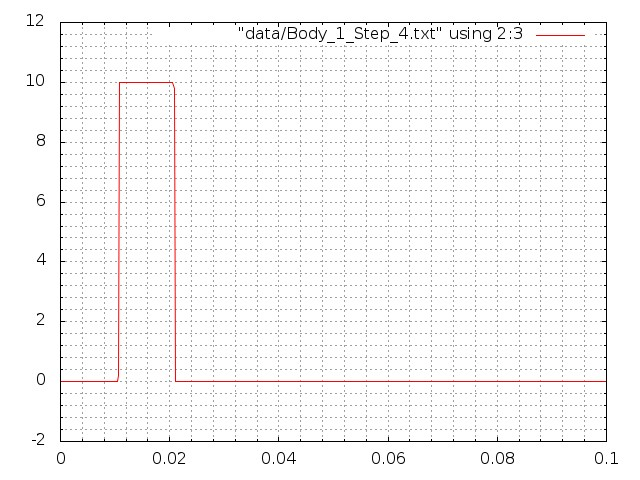
\includegraphics[width=1\linewidth]{png/1d/el-non-mv.png}} a) \\
\end{minipage}
\hfill
\begin{minipage}[h]{0.47\linewidth}
\center{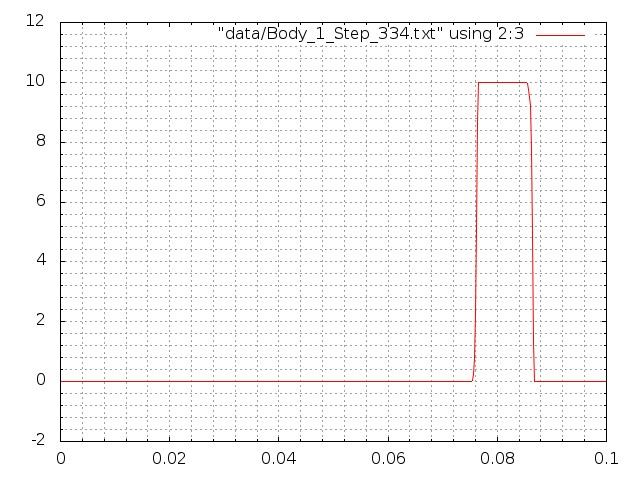
\includegraphics[width=1\linewidth]{png/1d/el-non-mv-2.png}} \\b)
\end{minipage}
\vfill
\begin{minipage}[h]{0.47\linewidth}
\center{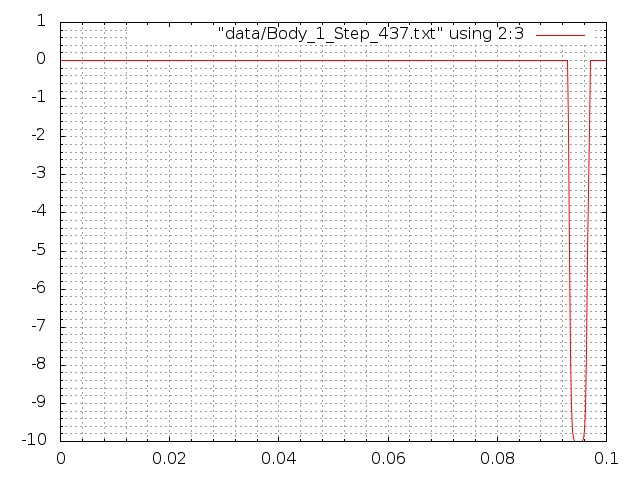
\includegraphics[width=1\linewidth]{png/1d/el-non-mv-2,5.png}} c) \\
\end{minipage}
\hfill
\begin{minipage}[h]{0.47\linewidth}
\center{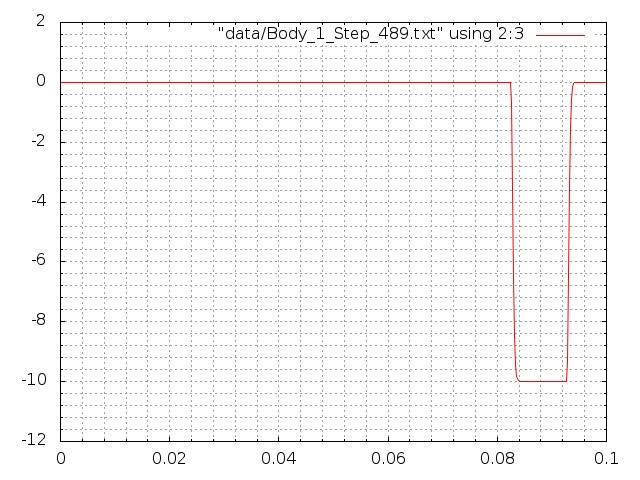
\includegraphics[width=1\linewidth]{png/1d/el-non-mv-3.png}} d) \\
\end{minipage}
\caption{Распространение прямоугольного импульса, неподвижная сетка a) начальное возмущение, b)
импульс прошёл через всё тело, c) отражение от закреплённой границы, d) Отражённый импульс.}
\label{pic:el-non-mv}
\end{figure}

\subparagraph{Подвижная сетка}
В силу равенства нулю правой части и неподвижности сетки вышеизложенный метод абсолютно точен по времени. В случае движения сетки возникают проблемы с порядком точности по времени, которые решаются более симметричным расщеплением процессов распространения возмущения и переноса вещества, описанным в .

На рис.\ref{pic:el-mv} показано отражение упругой волны от свободной границы (граничное условие $\sigma = 0$,       скорость сохраняет знак). Благодаря расщеплению размытие фронта остаётся таким же, как и в методе на неподвижной сетке.

\begin{figure}
\begin{minipage}[h]{0.47\linewidth}
\center{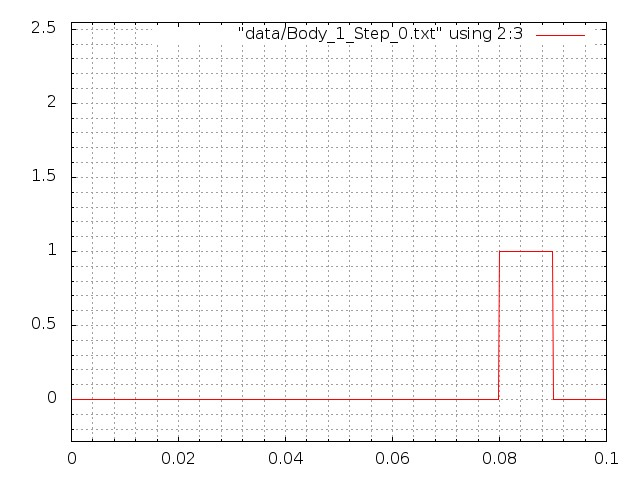
\includegraphics[width=1\linewidth]{png/1d/el-mv.png}} a) \\
\end{minipage}
\hfill
\begin{minipage}[h]{0.47\linewidth}
\center{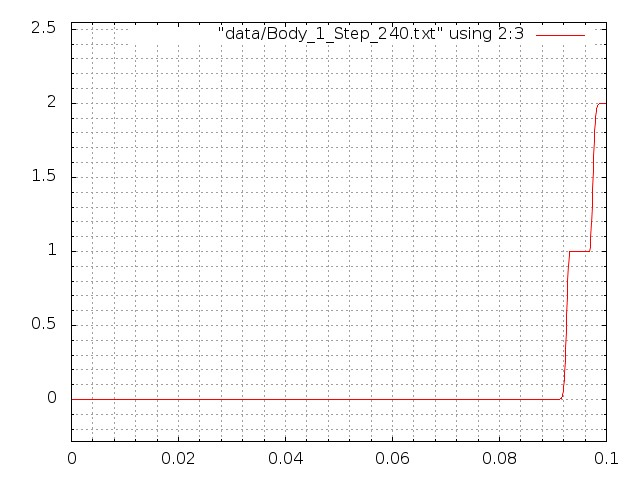
\includegraphics[width=1\linewidth]{png/1d/el-mv-2.png}} \\b)
\end{minipage}
\vfill
\begin{minipage}[h]{0.47\linewidth}
\center{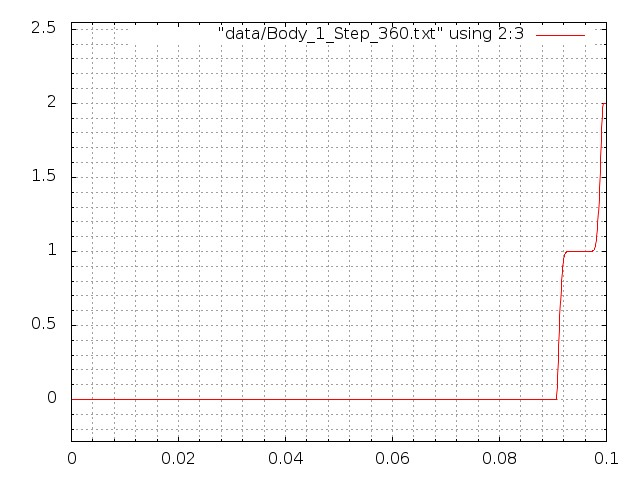
\includegraphics[width=1\linewidth]{png/1d/el-mv-3.png}} c) \\
\end{minipage}
\hfill
\begin{minipage}[h]{0.47\linewidth}
\center{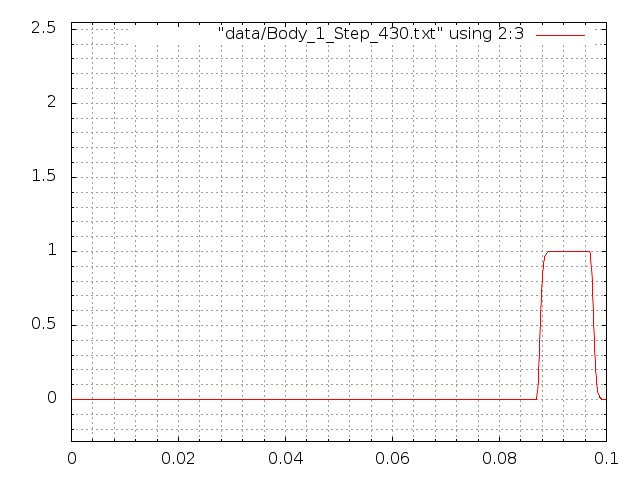
\includegraphics[width=1\linewidth]{png/1d/el-mv-4.png}} d) \\
\end{minipage}
\caption{Распространение прямоугольного импульса, подвижная сетка a) начальное возмущение, b,c) отражение от свободной границы, d) Отражённый импульс.}
\label{pic:el-mv}
\end{figure}

\subparagraph{Ударная волна}
Подвижность сетки позволяет получать гораздо более реальные результаты -- к примеру, в случае достаточно больших скоростей начальных возмущений, независимо от их гладкости, в материале образуется ударная волна (рис.\ref{pic:udarnaya-volna}).

\begin{figure}
\begin{minipage}[h]{0.47\linewidth}
\center{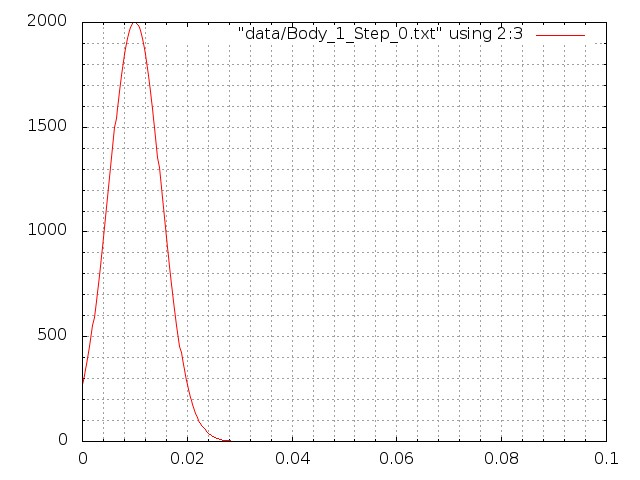
\includegraphics[width=1\linewidth]{png/1d/ud-volna.png}} a) \\
\end{minipage}
\hfill
\begin{minipage}[h]{0.47\linewidth}
\center{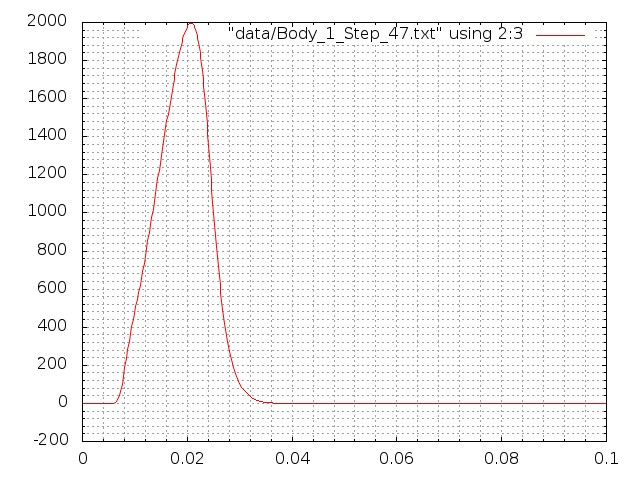
\includegraphics[width=1\linewidth]{png/1d/ud-volna-2.png}} \\b)
\end{minipage}
\vfill
\begin{minipage}[h]{0.47\linewidth}
\center{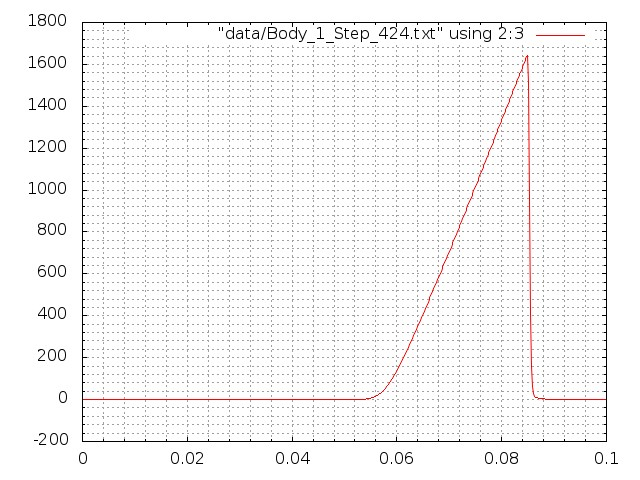
\includegraphics[width=1\linewidth]{png/1d/ud-volna-3.png}} c) \\
\end{minipage}
\hfill
\begin{minipage}[h]{0.47\linewidth}
\center{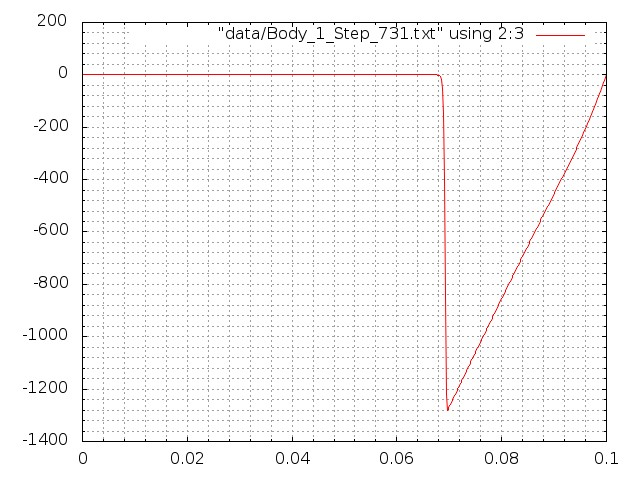
\includegraphics[width=1\linewidth]{png/1d/ud-volna-4.png}} d) \\
\end{minipage}
\caption{Формирование ударной волны при гладком начальном условии a) начальное возмущение - гауссова кривая, b,c) опрокидывание фронта, d) отражённый импульс.}
\label{pic:udarnaya-volna}
\end{figure}

\subparagraph{Расчёт слоистой структуры}
Также в работе был произведён расчёт прохождения возмущения через многослойную структуру с возрастающей от слоя к слою плотностью. На рис.\ref{pic:mnogosloika} показаны значения скорости в частицах материала по мере прохождения в новые слои.

\begin{figure}
\begin{minipage}[h]{0.47\linewidth}
\center{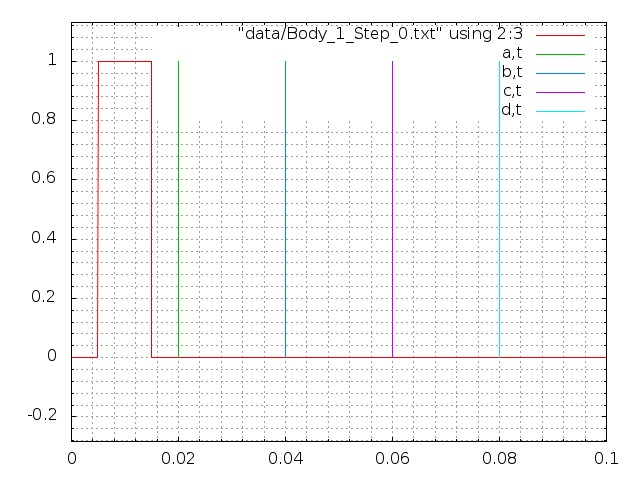
\includegraphics[width=1\linewidth]{png/1d/mnogosloika.png}}  \\
\end{minipage}
\hfill
\begin{minipage}[h]{0.47\linewidth}
\center{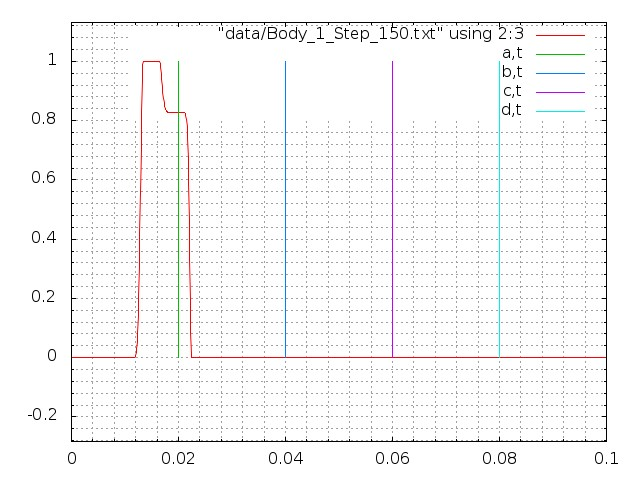
\includegraphics[width=1\linewidth]{png/1d/mnogosloika-2.png}} \\
\end{minipage}
\vfill
\begin{minipage}[h]{0.47\linewidth}
\center{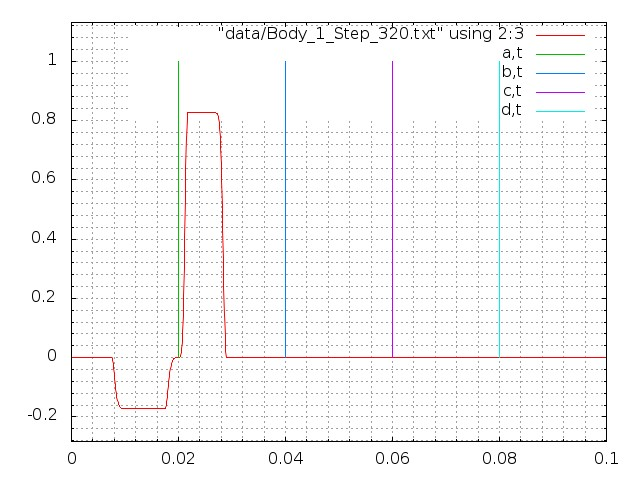
\includegraphics[width=1\linewidth]{png/1d/mnogosloika-3.png}}  \\
\end{minipage}
\hfill
\begin{minipage}[h]{0.47\linewidth}
\center{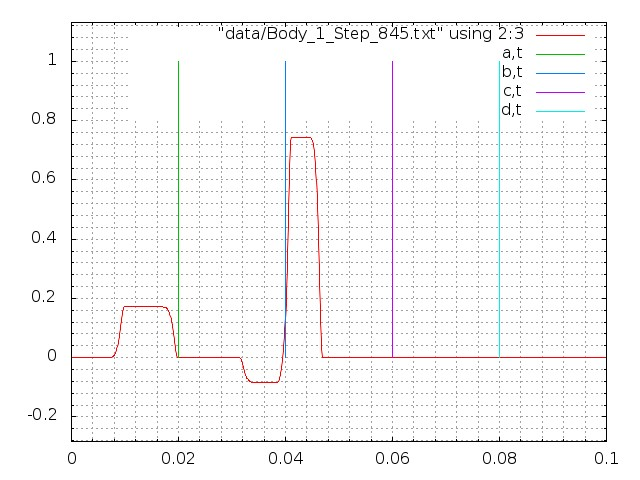
\includegraphics[width=1\linewidth]{png/1d/mnogosloika-4.png}}  \\
\end{minipage}
\vfill
\begin{minipage}[h]{0.47\linewidth}
\center{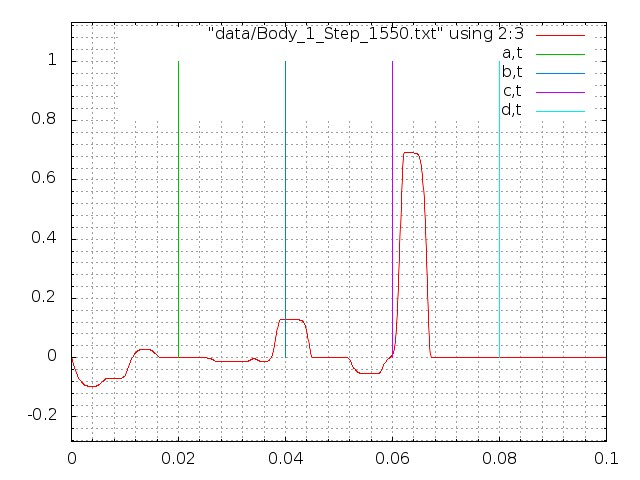
\includegraphics[width=1\linewidth]{png/1d/mnogosloika-5.png}} \\
\end{minipage}
\hfill
\begin{minipage}[h]{0.47\linewidth}
\center{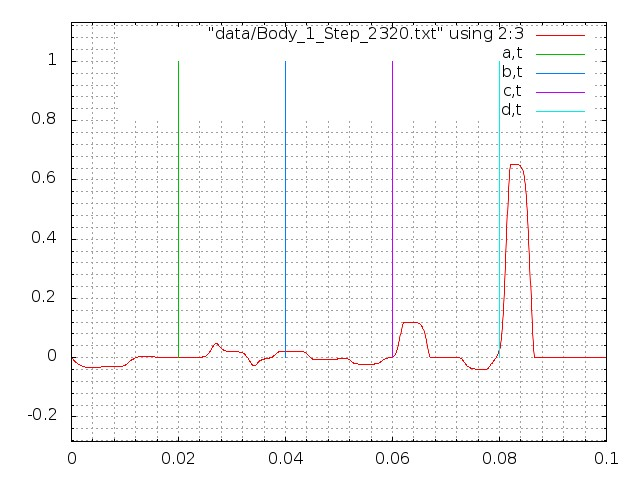
\includegraphics[width=1\linewidth]{png/1d/mnogosloika-6.png}} \\
\end{minipage}
\caption{Прохождение упругой волны через слоистый материал.}
\label{pic:mnogosloika}
\end{figure}

Сравнение численных расчётов с аналитическими результатами, изложенными в \cite{petrov_tormasov_holodov}, показало их совпадение с высокой (относительная ошибка $10^{-10}$ во втором слое и $10^{-3}$ в пятом) точностью.

\subsubsection{Упругопластика}
Для случая упругопластики в одномерном случае была использована модель с кусочно-линейным по напряжению модулем Юнга (производной $\frac{d\sigma}{d\varepsilon}$) и однозначной зависимостью $\sigma-\varepsilon$. Распространение пластического возмущения показано на рис.\ref{pic:plastic-1d}.

\begin{figure}
\begin{minipage}[h]{0.47\linewidth}
\center{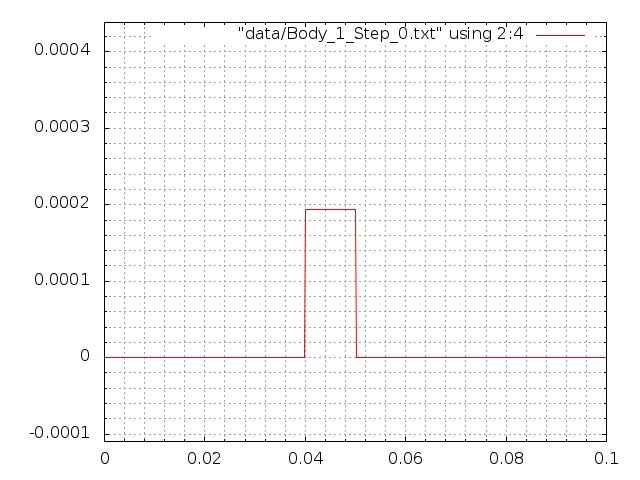
\includegraphics[width=1\linewidth]{png/1d/plastic-1d.png}} a) \\
\end{minipage}
\hfill
\begin{minipage}[h]{0.47\linewidth}
\center{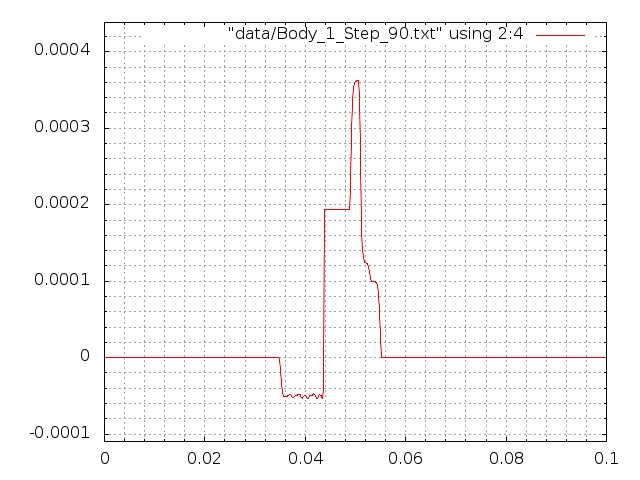
\includegraphics[width=1\linewidth]{png/1d/plastic-1d-2.png}} \\b)
\end{minipage}
\vfill
\begin{minipage}[h]{0.47\linewidth}
\center{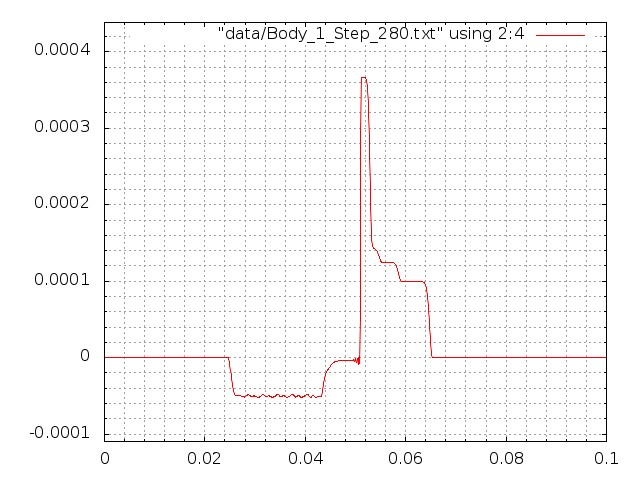
\includegraphics[width=1\linewidth]{png/1d/plastic-1d-3.png}} c) \\
\end{minipage}
\hfill
\begin{minipage}[h]{0.47\linewidth}
\center{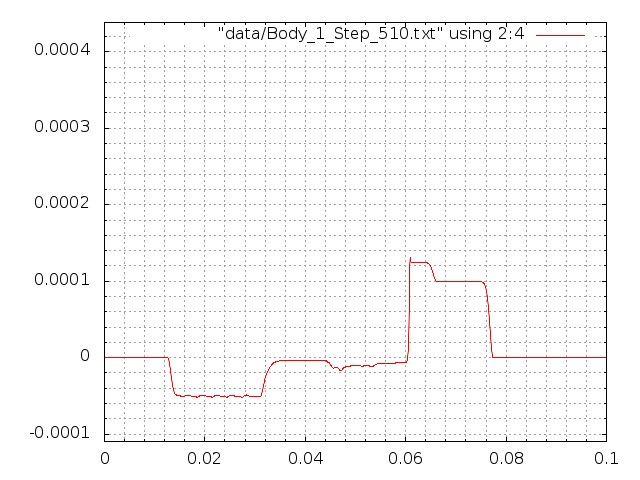
\includegraphics[width=1\linewidth]{png/1d/plastic-1d-4.png}} d) \\
\end{minipage}
\caption{Пластические возмущения a) начальное возмущение - прямоугольник, b) влево уходит чисто упругая волна, справа образуются "упругие предвестники", c) отчётливые четыре "ступеньки" в пластической волне, d) пластическая волна переходит в упругую.}
\label{pic:plastic-1d}
\end{figure}

Четыре "ступеньки" в пластической волне обусловлены четыремя различными значениями модуля Юнга, и, соответственно, скоростями распространения $c = \sqrt{\frac{E}{\rho}}$. Значения напряжений в них совпадают с максимальным верхним пределом, при котором модуль Юнга всё ещё имеет соответствующее значение.

\subsubsection{Неявный метод}
В рамках одномерного кода был также реализован неявный метод второго порядка на неподвижной сетке, описанный в \cite{kukudganov}, стр. 183, являющийся абсолютно устойчивым по времени. Однако практика показала, что он менее пригоден для моделирования динамических процессов ввиду ряда недостатков:
\begin{itemize}
\item Общая сложность реализации, которая вряд ли позволит применить метод в трёхмерном случае
\item Автору неизвестен метод распараллеливания на произвольное число процессов
\item Существенно большее размытие фронтов и величина осцилляций, чем у явного метода второго порядка (см. рис.\ref{pic:implicit})
\item Несмотря на абсолютную устойчивость, при выборе большого шага по времени смоделированная картина перестаёт соответствовать действительности
\end{itemize}
Возможно, данный метод будет полезен для статических расчётов, в которых не важна кратковременная волновая картина и требуется расчёт на существенно больших временах.

\begin{figure}
\begin{minipage}[h]{0.47\linewidth}
\center{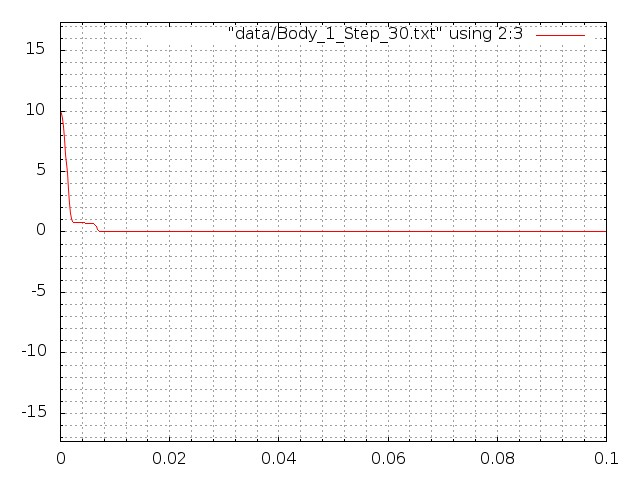
\includegraphics[width=1\linewidth]{png/1d/implicit.png}} \\
\end{minipage}
\hfill
\begin{minipage}[h]{0.47\linewidth}
\center{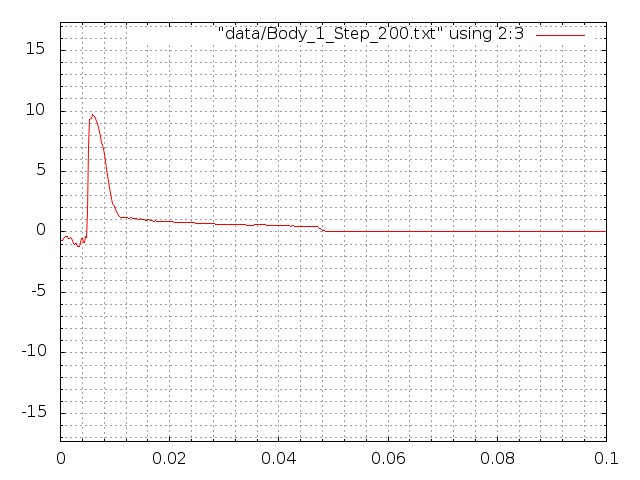
\includegraphics[width=1\linewidth]{png/1d/implicit-2.png}} \\
\end{minipage}
\vfill
\begin{minipage}[h]{0.47\linewidth}
\center{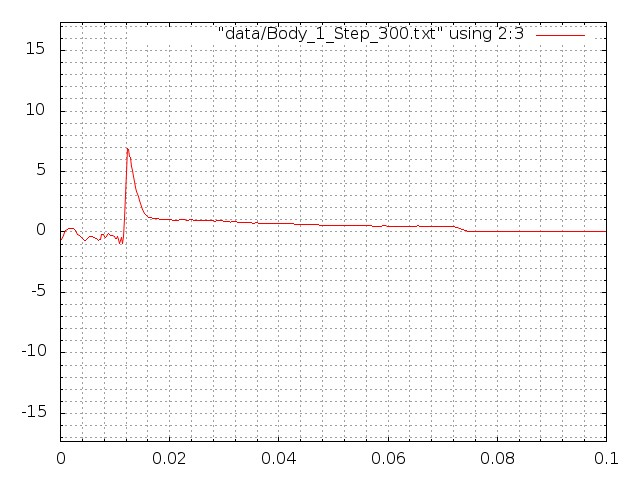
\includegraphics[width=1\linewidth]{png/1d/implicit-3.png}} \\
\end{minipage}
\hfill
\begin{minipage}[h]{0.47\linewidth}
\center{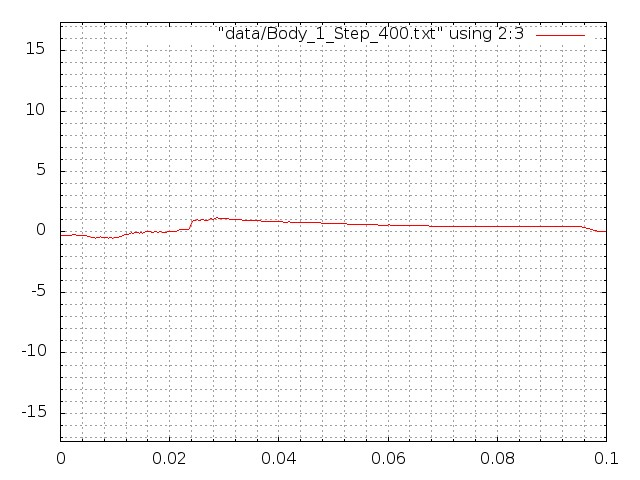
\includegraphics[width=1\linewidth]{png/1d/implicit-4.png}} \\
\end{minipage}
\caption{Боковой удар по телу с пластической реологией. Расчёт неявным методом второго порядка со сглаживанием}
\label{pic:implicit}
\end{figure}

\subsection{Расчёты в 3D}
Для трёхмерной модели сплошной среды на основе существующего программного комплекса, поддерживающего расчёт  линейно-упругой реологии, был реализован расчёт упругопластической реологии на основе теории пластического течения с критерием текучести Мизеса. Расчёт был проведён на кубической (рис. \ref{pic:mesh},a) и тетраэдрической сетках (рис. \ref{pic:mesh},b)
\begin{figure}
\begin{minipage}{0.8\linewidth}
\center{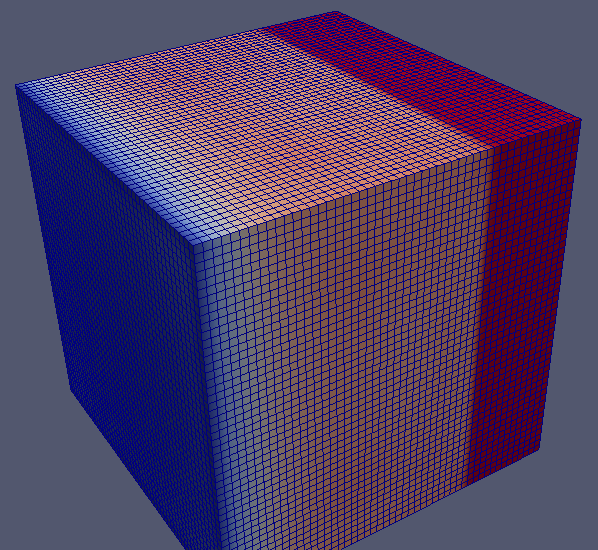
\includegraphics[width=1\linewidth]{png/3d/cubic-mesh.png}} a)\\
\end{minipage}
\vfill
\begin{minipage}{0.8\linewidth}
\center{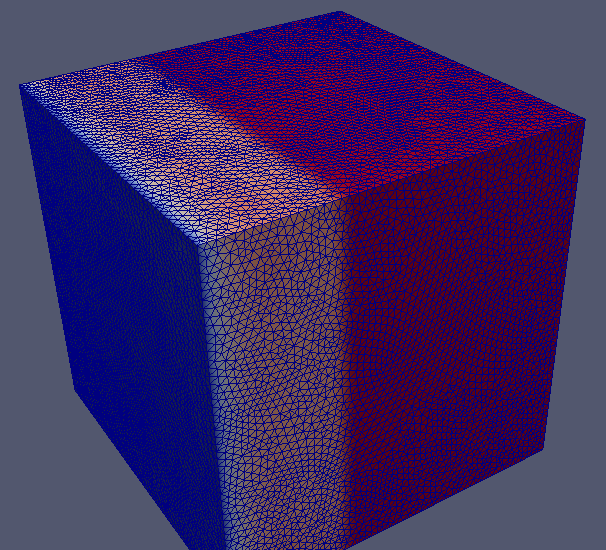
\includegraphics[width=1\linewidth]{png/3d/tetr-mesh.png}} b)\\
\end{minipage}
\caption{Вид рассчётной сетки: a) кубическая, b) тетраэдрическая}
\label{pic:mesh}
\end{figure}

\subsubsection{Расчёт бокового удара по телу упругопластической реологии}
Смоделирован удар по телу пластической реологии типа металла. 

"Удар" представляет собой граничное условие фиксированного напряжения, превышающего предел текучести материала, конечной или бесконечной длительности по времени. Характерный вид возмущения в 3D можно видеть на рис.\ref{pic:mesh}. 

На рис.\ref{pic:pl-wave} показаны волны напряжений (в направлении прямой вдоль удара), возникшие от сильного бокового удара по модельному кубику. Можно видеть быструю волну, распространяющуюся со скоростью звука и по амплитуде равной пределу текучести материала -- "упругий предвестник". За ним с меньшей скоростью распространяется пластическая волна. 

Из рисунка видны различия решения при расчётах на кубических и тетраэдрических сетках. К преимуществам кубической сетки можно отнести большую быстроту счёта при той же мелкости и меньшее размывание фронтов. Однако для сложных форм тел и начальных возмущений целесообразнее применять тетраэдрическую сетку, которая намного лучше заполняет рассчётную область и не создаёт численной анизотропии решения.

\begin{figure}
\begin{minipage}{0.35\linewidth}
\center{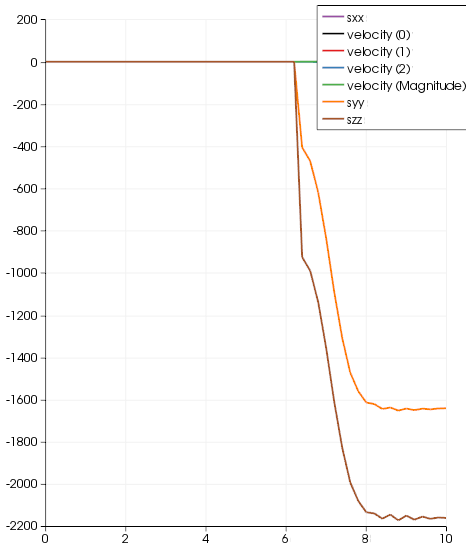
\includegraphics[width=1\linewidth]{png/3d/cubic-19-02-s.png}} a)\\
\end{minipage}
\hfill
\begin{minipage}{0.35\linewidth}
\center{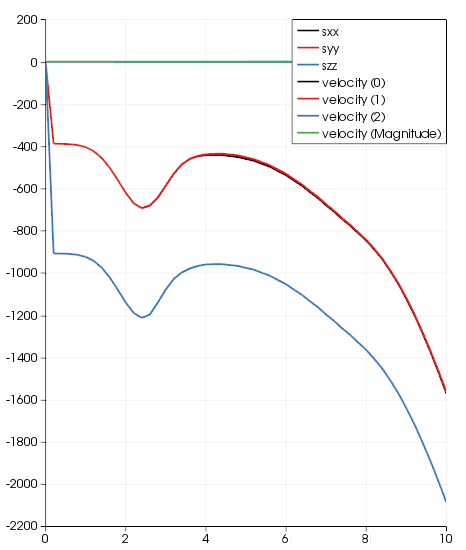
\includegraphics[width=1\linewidth]{png/3d/cubic-50-02-s.png}} b)\\
\end{minipage}
\vfill
\begin{minipage}{0.35\linewidth}
\center{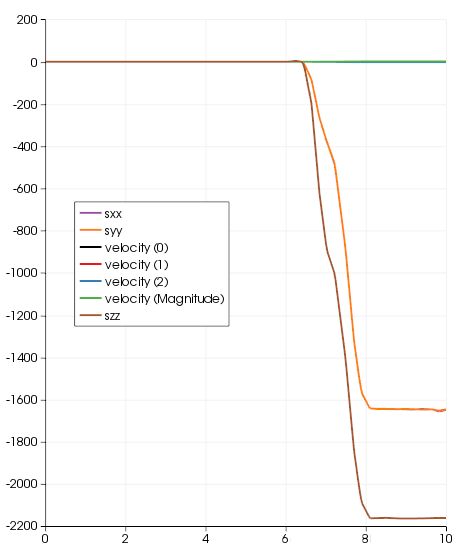
\includegraphics[width=1\linewidth]{png/3d/tetr-50-02-s.png}} c)\\
\end{minipage}
\hfill
\begin{minipage}{0.35\linewidth}
\center{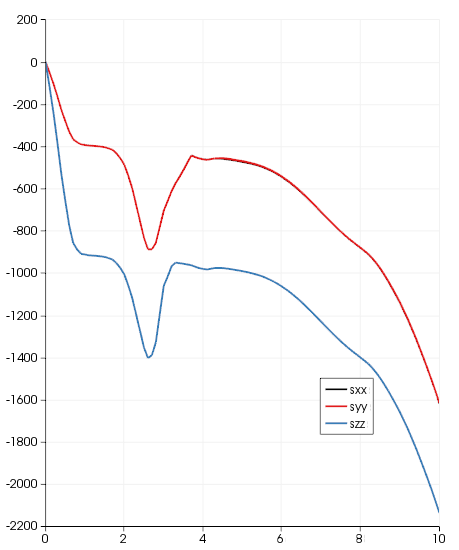
\includegraphics[width=1\linewidth]{png/3d/tetr-150-02-s.png}} d)\\
\end{minipage}
\caption{Профиль волны от бокового удара по стальному кубику. a,b - кубическая, c,d - тетраэдрическая сетки}
\label{pic:pl-wave}
\end{figure}

На рис.\ref{pic:pl-strike-2d} показан двумерный срез куба, по которому нанесён боковой удар конечной длительности. Заметно отрицательное влияние отражённых от границы волн, размывающих интересующее плоское решение.

\begin{figure}
\begin{minipage}{0.3\linewidth}
\center{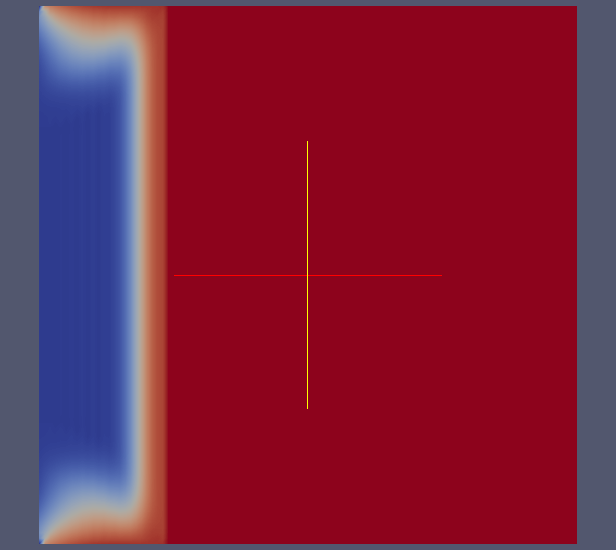
\includegraphics[width=1\linewidth]{png/3d/plastic-strike-1.png}} a)\\
\end{minipage}
\hfill
\begin{minipage}{0.3\linewidth}
\center{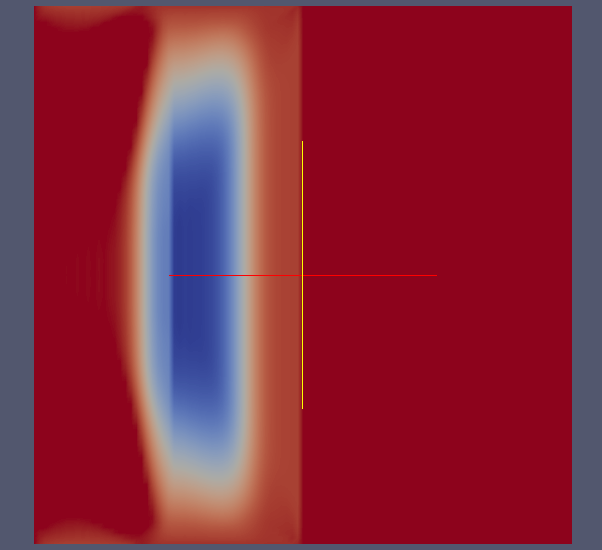
\includegraphics[width=1\linewidth]{png/3d/plastic-strike-2.png}} b)\\
\end{minipage}
\hfill
\begin{minipage}{0.3\linewidth}
\center{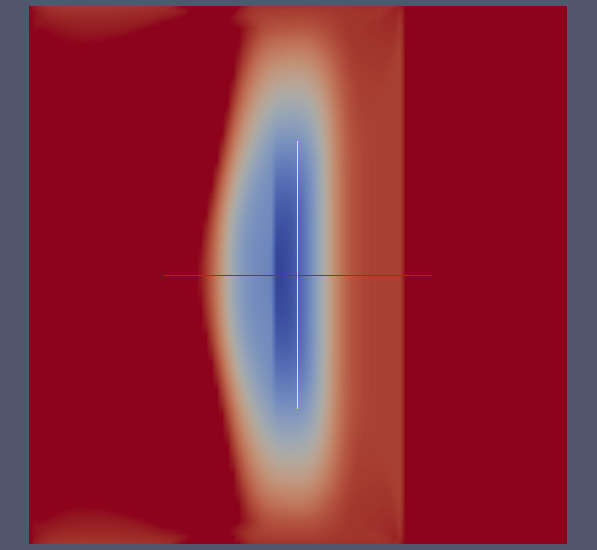
\includegraphics[width=1\linewidth]{png/3d/plastic-strike-3.png}} c)\\
\end{minipage}
\caption{Профиль волны от бокового удара конечной длительности. a,b,c - последовательные моменты времени}
\label{pic:pl-strike-2d}
\end{figure}

Более детально результаты удара конечной длительности позволяет рассмотреть одномерный рис.\ref{pic:pl-strike-1d}, на котором видна волна разгрузки (волна Рахматулина), следующая за пластическим возмущением. Амплитуда волны упругой разгрузки, отсчитанная от амплитуды пластичекой волны, в два раза превышает амплитуду упругого предвестника, что соответствует аналитическому рассмотрению одномерной волны Рахматулина \cite{wilkins}.

\begin{figure}
\begin{minipage}{0.3\linewidth}
\center{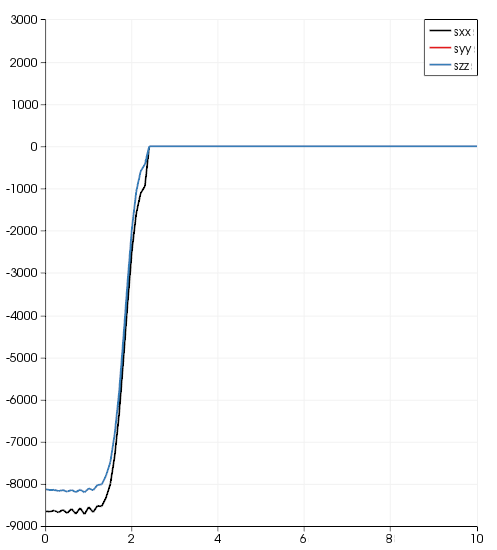
\includegraphics[width=1\linewidth]{png/3d/plastic-strike-1d-1.png}} a)\\
\end{minipage}
\hfill
\begin{minipage}{0.3\linewidth}
\center{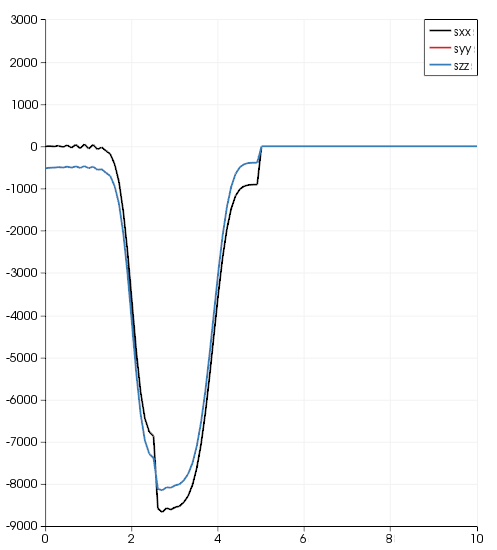
\includegraphics[width=1\linewidth]{png/3d/plastic-strike-1d-2.png}} b)\\
\end{minipage}
\hfill
\begin{minipage}{0.3\linewidth}
\center{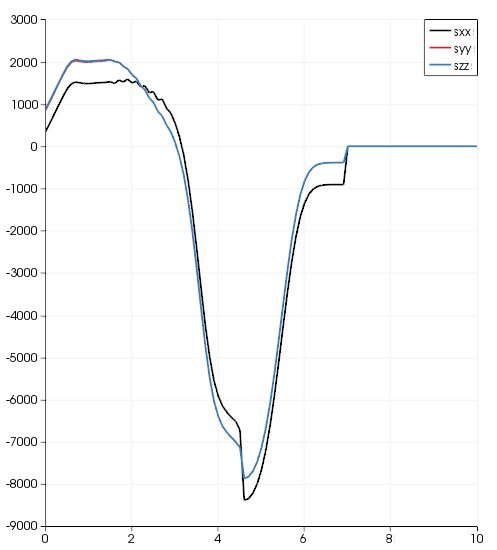
\includegraphics[width=1\linewidth]{png/3d/plastic-strike-1d-3.png}} c)\\
\end{minipage}
\caption{Профиль волны от бокового удара конечной длительности. Значения напряжений в направлении прямой вдоль удара. a,b,c - последовательные моменты времени}
\label{pic:pl-strike-1d}
\end{figure}

\subsubsection{Расчёт прохождения пластической волны через контакт двух материалов}
В рамках расчёта слоистых структур при динамических нагрузках было смоделировано прохождение упругопластической волны через контакт двух тестовых материалов с отличающейся в четыре раза плотностью. 

На рис.\ref{pic:two-materials} показано в косом срезе испытуемое двухслойное тело.

\begin{figure}[H]
\center{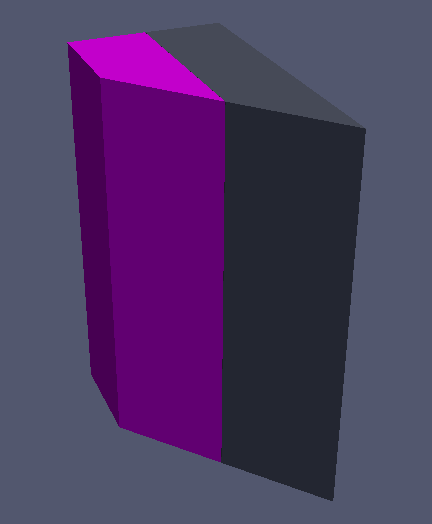
\includegraphics[width=0.5\linewidth]{png/3d/contact/two-materials}}
\caption{Косой срез тела, по которому наносится боковой удар. Разными цветами показаны разные материалы}
\label{pic:two-materials}
\end{figure} 

Ниже (рис.\ref{pic:two-mat-3d}) показан вид возмущения (компонента тензора напряжений в направлении удара $\sigma_{xx}$) в трёхмерном пространстве. Синему цвету соответствуют высокие отрицательные напряжения, красному -- положительные.

\begin{figure}
\begin{minipage}{0.4\linewidth}
\center{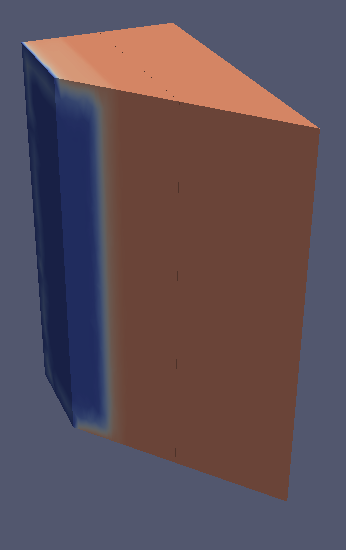
\includegraphics[width=1\linewidth]{png/3d/contact/3d-1.png}} a)\\
\end{minipage}
\hfill
\begin{minipage}{0.4\linewidth}
\center{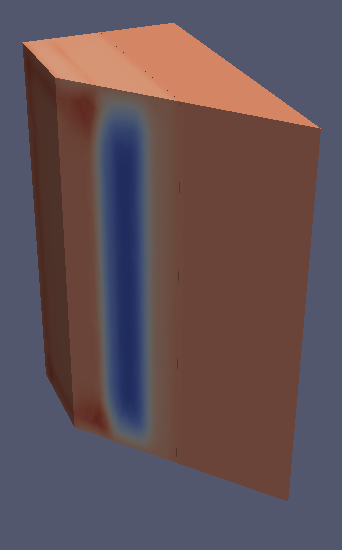
\includegraphics[width=1\linewidth]{png/3d/contact/3d-2.png}} b)\\
\end{minipage}
\vfill
\begin{minipage}{0.4\linewidth}
\center{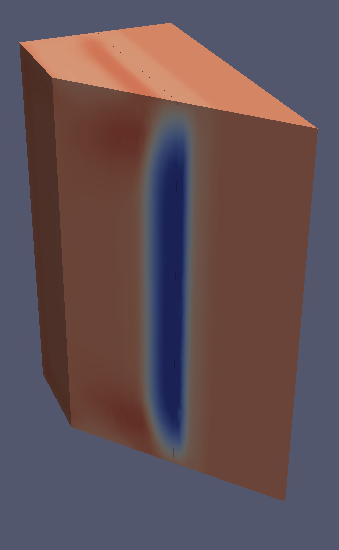
\includegraphics[width=1\linewidth]{png/3d/contact/3d-3.png}} c)\\
\end{minipage}
\hfill
\begin{minipage}{0.4\linewidth}
\center{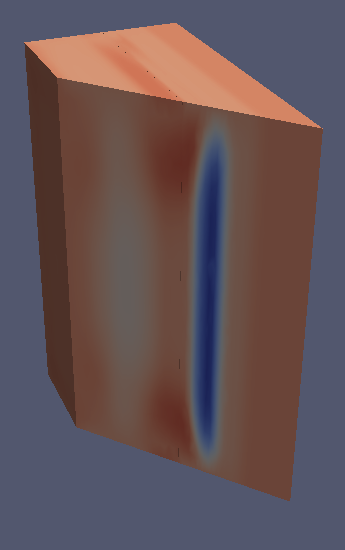
\includegraphics[width=1\linewidth]{png/3d/contact/3d-4.png}} d)\\
\end{minipage}
\caption{Прохождение упругопластической волны через контакт (полное слипание) в 3D (цветом показаны значения $\sigma_{xx}$)}
\label{pic:two-mat-3d}
\end{figure}

Сравнение решения с учётом пластической реологии с решением в чисто упругой постановке проведено на двумерном срезе вдоль направления удара на рис.\ref{pic:plastic-vs-elastic} и на одномерных графиках (рис.\ref{pic:el-contact} и \ref{pic:pl-contact}) напряжений вдоль направления удара.

\begin{figure}
\begin{minipage}[h]{0.47\linewidth}
\center{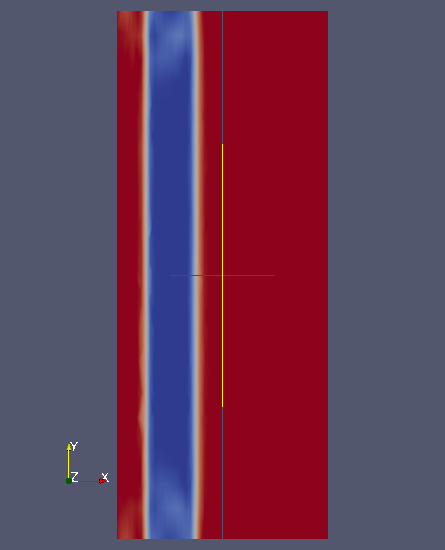
\includegraphics[width=0.7\linewidth]{png/3d/contact/el-vs-contact-1.png}}  \\
\end{minipage}
\hfill
\begin{minipage}[h]{0.4\linewidth}
\center{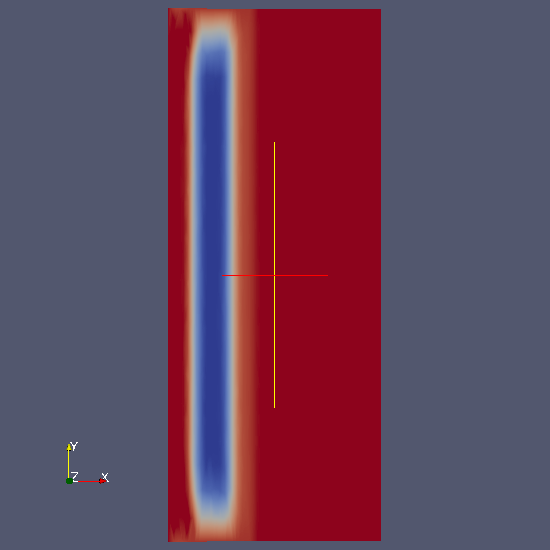
\includegraphics[width=1\linewidth]{png/3d/contact/pl-vs-contact-1.png}} \\
\end{minipage}
\vfill
\begin{minipage}[h]{0.47\linewidth}
\center{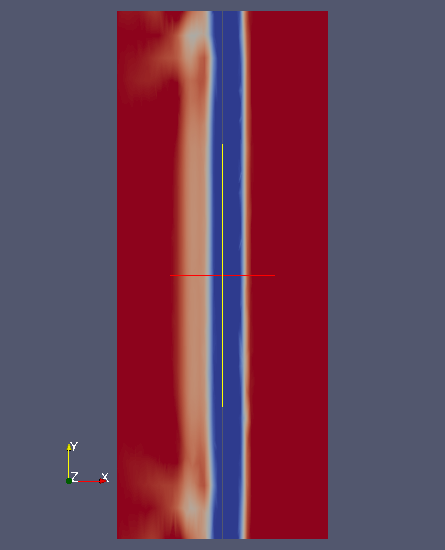
\includegraphics[width=0.7\linewidth]{png/3d/contact/el-vs-contact-2.png}}  \\
\end{minipage}
\hfill
\begin{minipage}[h]{0.4\linewidth}
\center{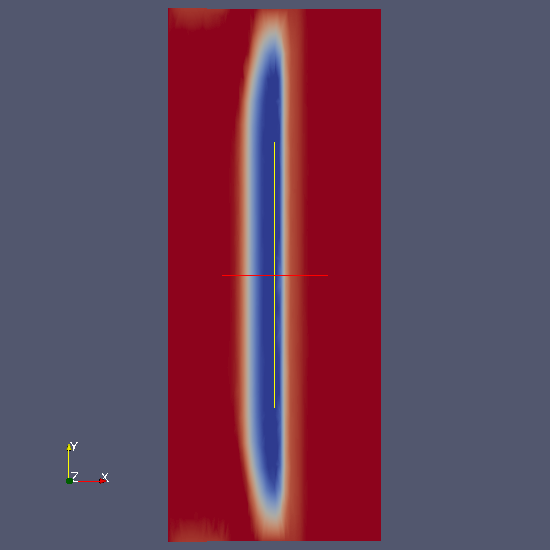
\includegraphics[width=1\linewidth]{png/3d/contact/pl-vs-contact-2.png}}  \\
\end{minipage}
\vfill
\begin{minipage}[h]{0.47\linewidth}
\center{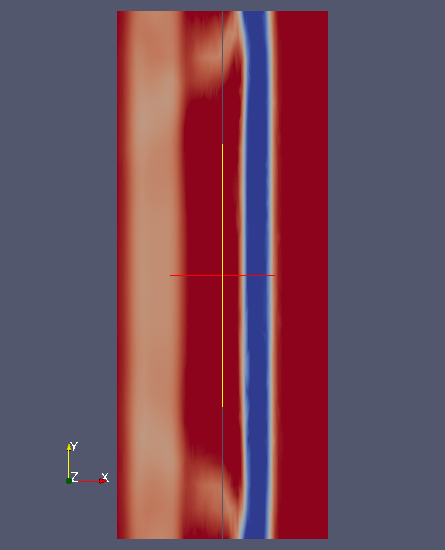
\includegraphics[width=0.7\linewidth]{png/3d/contact/el-vs-contact-3.png}} \\
\end{minipage}
\hfill
\begin{minipage}[h]{0.4\linewidth}
\center{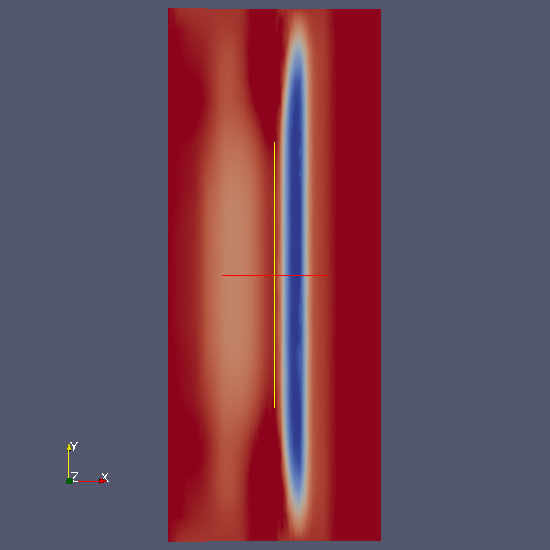
\includegraphics[width=1\linewidth]{png/3d/contact/pl-vs-contact-3.png}} \\
\end{minipage}
\caption{Сравнение отклика тел с линейно-упругой (слева) и упругопластической (справа) реологией на одинаковое начальное возмущение}
\label{pic:plastic-vs-elastic}
\end{figure}

\begin{figure}
\begin{minipage}{0.35\linewidth}
\center{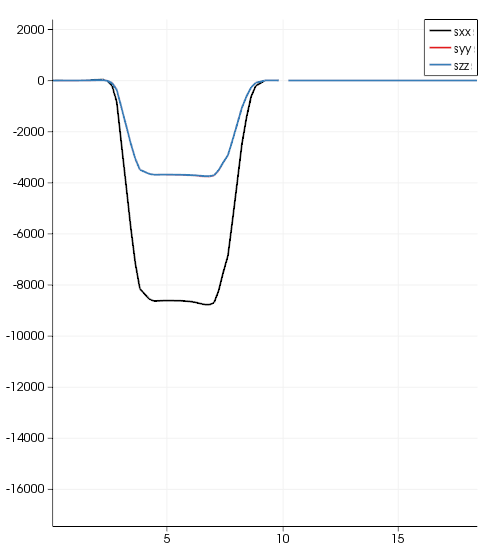
\includegraphics[width=1\linewidth]{png/3d/contact/elastic-contact-1.png}} a)\\
\end{minipage}
\hfill
\begin{minipage}{0.35\linewidth}
\center{\includegraphics[width=1\linewidth]{png/3d/contact/elastic-contact-2.png}} b)\\
\end{minipage}
\caption{Прохождение упругой волны через контакт двух материалов: a) до прохождения контакта, b) после}
\label{pic:el-contact}
\end{figure}

\begin{figure}
\begin{minipage}{0.35\linewidth}
\center{\includegraphics[width=1\linewidth]{png/3d/contact/plastic-contact-1.png}} a)\\
\end{minipage}
\hfill
\begin{minipage}{0.35\linewidth}
\center{\includegraphics[width=1\linewidth]{png/3d/contact/plastic-contact-2.png}} b)\\
\end{minipage}
\vfill
\begin{minipage}{0.35\linewidth}
\center{\includegraphics[width=1\linewidth]{png/3d/contact/plastic-contact-3.png}} c)\\
\end{minipage}
\hfill
\begin{minipage}{0.35\linewidth}
\center{\includegraphics[width=1\linewidth]{png/3d/contact/plastic-contact-4.png}} d)\\
\end{minipage}
\caption{Прохождение упругопластической волны через контакт двух материалов, последовательные моменты времени}
\label{pic:pl-contact}
\end{figure}

Помимо отличий чисто упругой волны от упругопластической, проявляющихся в наличии у первой упругого предвестника, волны упругой разгрузки и, собственно, пластической волны, имеются отличия, связанные с прохождением контакта. 

Амплитуда напряжений прошедшей в более плотный слой волны не возрастает, что обусловлено наличием предела текучести, одинакового в обоих материалах. В профиле отражённой волны появляются области, где компоненты напряжений, перпендикулярные направлению распространения, превосходят нормальную компоненту.

Несмотря на простоту используемой модели, в расчётах удалось получить многие известные эффекты для упругопластических материалов.